\documentclass[10pt,reqno]{amsart}
\usepackage[T1]{fontenc}\usepackage[utf8]{inputenc}\usepackage{lmodern}
\usepackage[a4paper,margin=26mm]{geometry}
\usepackage{amsmath,amssymb,mathtools,booktabs,microtype,tikz}
\usepackage[hidelinks]{hyperref}
\newtheorem{theorem}{Theorem}\newtheorem{lemma}[theorem]{Lemma}
\title{Factor-sum returns and fixed-tail Pell fibres for rational Erd\H{o}s--Straus traces}
\author{The Clankers}\date{22 September 2026}
\begin{document}
\begin{abstract}
An original middle trace at a prime-square distinguished denominator can have
integral tail sum while every full gate at its shell, and every fixed-word or
fixed-ray residual-divisor return, fails. We prove an explicit different
return preserving the sum of two factors of the distinguished denominator.
Its entire domain and inverse are given by one quadratic equation. The
prime-square specialization is Pell, with an explicit infinite integer family
and independently certified hard-prime examples. A square-zero coordinate also
allows genuinely mixed E/M cancellation inside the unchanged original exponent
box. A second exact Pell lattice classifies every integral target that retains
the numerical tail sum. For every proper prime-square trace, no such target
can have residual a proper divisor of the source residual. At $p=67369$ the
complete fibre is empty for every proper original trace sum. No universal
source-existence assertion is made.
\end{abstract}\maketitle

Let $p\equiv1\pmod4$ be prime, $p/4<a<p/2$, $R=4a-p$, and $u\mid a^2$.
With $g=\gcd(a,u)$ and $(h,r,s)=(g^2/u,u/g,a/g)$, retain
\begin{align*}
 E:&\quad(a,hs\kappa,phr\kappa),&\kappa&=(pr+s)/R,\\
 M:&\quad(a,phs\lambda,phr\lambda),&\lambda&=(r+s)/R.
\end{align*}
These are rational reciprocal identities. Their full integer gates are
$R\mid4u+1$ and $R\mid p+4u$; integral tail sum requires their squares
instead. The ordered divisor inverses are $a^2/(Ry-pa)$ and $pa^2/(Ry-pa)$.
These inherited Type-I/II coordinates are reviewed in Elsholtz and Tao [1,
\S2]. We retain the complete box $0\le v_\ell(u)\le2v_\ell(a)$.

\begin{lemma}[Prime-square terminal trace]
Suppose $p\equiv1\pmod{24}$ and $a=q^2$, $q>3$ prime. Every M trace has
$u=q$ or $q^3$, $R\mid(q+1)^2$. If $R\nmid q+1$, its whole original shell
has no full E/M state. Neither word, nor either primitive M ray, admits any
proper residual-divisor return preserving that word or ray.
\end{lemma}
\begin{proof}
One has $R\equiv3\pmod{24}$. Reduction of the square gates modulo three forces
$q\equiv2\pmod3$ and odd word exponent; hence only $q,q^3$ occur. The two
M square gates are equivalent to $R\mid(q+1)^2$.
Write $K=\prod_{\ell^e\parallel R}\ell^{\lceil e/2\rceil}$.
If an E trace also occurred, $q\equiv-1\pmod K$ would give
$K\mid4q^f+1\equiv-3\pmod K$ for its odd $f$. This forces $R=3$,
incompatible with properness. Both M words are nonintegral by assumption.

A deletion to $R/k$ retaining $u=q$ or either primitive M ray requires
$k\mid R$, $k>1$, $k\equiv1\pmod{4q}$. Such $k$ divides $(q+1)^2$.
Its complement $v=(q+1)^2/k$ exceeds one (otherwise $k$ is even), and is
one modulo $q$. Writing $k=1+qA$, $v=1+qB$ gives $A\ge4$, $B\ge1$ and
$qAB+A+B=q+2$, impossible. For the other word $q^3$, the word-preservation
modulus is $4q^2>R$, which also excludes every proper $k$.
\end{proof}

\begin{theorem}[Factor-sum arrow]
Take an original M trace with $a=hs$, $u=h$, $r=1$, and
$R=4hs-p=\delta t^2$, where $\delta$ is squarefree. Thus
$\delta\equiv3\pmod4$ and $\delta t\mid s+1$.
Its factor-sum-preserving returns with residual $\delta$ are exactly
\[
 h'=h-\delta w,\quad s'=s+\delta w,\qquad
 \delta w^2+(s-h)w=(t^2-1)/4,\quad w\in\mathbb Z.
\]
Every integer root gives positive integers $h',s'$, an available word
$u'=h'\mid(h's')^2$, and the ordered identity
\[
 \boxed{\frac4p=\frac1{h's'}+
 \frac1{ph's'\lambda'}+\frac1{ph'\lambda'},\qquad
 \lambda'=(s'+1)/\delta.}
\]
For a proper trace, $h's'<hs$.
\end{theorem}
\begin{proof}
Expansion gives
$h's'=hs+\delta w(h-s)-\delta^2w^2$.
Thus the quadratic is exactly $4h's'-p=\delta$.
The target product $(p+\delta)/4$ and factor sum $h+s$ are positive, proving
positivity of both factors. The original $
\delta\mid s+1$ gives $\delta\mid s'+1$, so the target is the full M marking
$(h',1,s',\lambda')$. Multiplying its reciprocal sum by $ph's'\lambda'$
gives $p\lambda'+s'+1=(p+\delta)\lambda'=4h's'\lambda'$.
The first-half range follows from $3\le\delta<p$.
Properness implies $t>1$, hence $hs-h's'=\delta(t^2-1)/4>0$.
\end{proof}

The map is an explicit finite algorithm. Its discriminant is
$(h-s)^2+R-\delta$; test its integer square root and divisibility by
$2\delta$. There are at most two possible $w$.
Its full incoming fibre at a marked target $(p,\delta,h',s')$ consists of
integers
\[
 -h'/\delta<w<s'/\delta,
\]
for which $1+4w(s'-h')-4\delta w^2=t^2$ is a positive odd square,
$\delta t^2<p$, and $\delta t\mid s'-\delta w+1$.
Recover $h=h'+\delta w$, $s=s'-\delta w$, $R=\delta t^2$, and $u=h$.
These tests are necessary and sufficient by the same expansion; retaining
$w$ gives both inverse compositions. The other M orientation is restored
using the new word's complement in the new square-divisor box.

\subsection*{Pell specialization and an integer family}
For $h=s=q$, the quadratic is precisely
\[
 t^2-4\delta w^2=1.
\]
For any positive solution, any squarefree $\delta\equiv3\pmod4$ and $k\ge1$,
put
\[
 q=\delta tk-1,\quad p=4q^2-\delta t^2,
 \quad h'=q-\delta w,\quad s'=q+\delta w,\quad\lambda'=tk+w.
\]
All quantities in the boxed reciprocal identity are positive integers.
Indeed $q\ge\delta t-1$ gives $p>\delta t^2$; Pell gives
$t>2\sqrt\delta\,w$, hence $q>\delta w$; and
$\delta t\mid q+1$ supplies the original trace.
Its exact reduced tail denominator is $t/\gcd(t,k)$.
This proves an integer identity without asserting that either quadratic
parameter is prime.

For $\delta=3$, the recurrence
\[
 (t_{n+1},w_{n+1})=(7t_n+24w_n,\ 2t_n+7w_n),\qquad(t_0,w_0)=(1,0)
\]
preserves $t^2-12w^2=1$ and yields infinitely many such integer inputs.
The first two certified prime instances are
\[
\begin{array}{r|r|r|r|r|r}
t&w&k&q&p&(h',s',\lambda')\\\hline
7&2&4&83&27409&(77,89,30)\\
97&28&4&1163&5382049&(1079,1247,416).
\end{array}
\]
At the first, $R=147$, $a=6889$ is a terminal prime-square trace as above,
but the new word is $77$, the new primitive ray is $(1,89)$, and
\[
 \frac4{27409}=\frac1{6853}+\frac1{5635016310}+\frac1{63314790}.
\]
The construction changes both invariants held fixed by the failed maps.
No infinitude of prime values in the Pell family is claimed.

\begin{figure}[htbp]
\centering
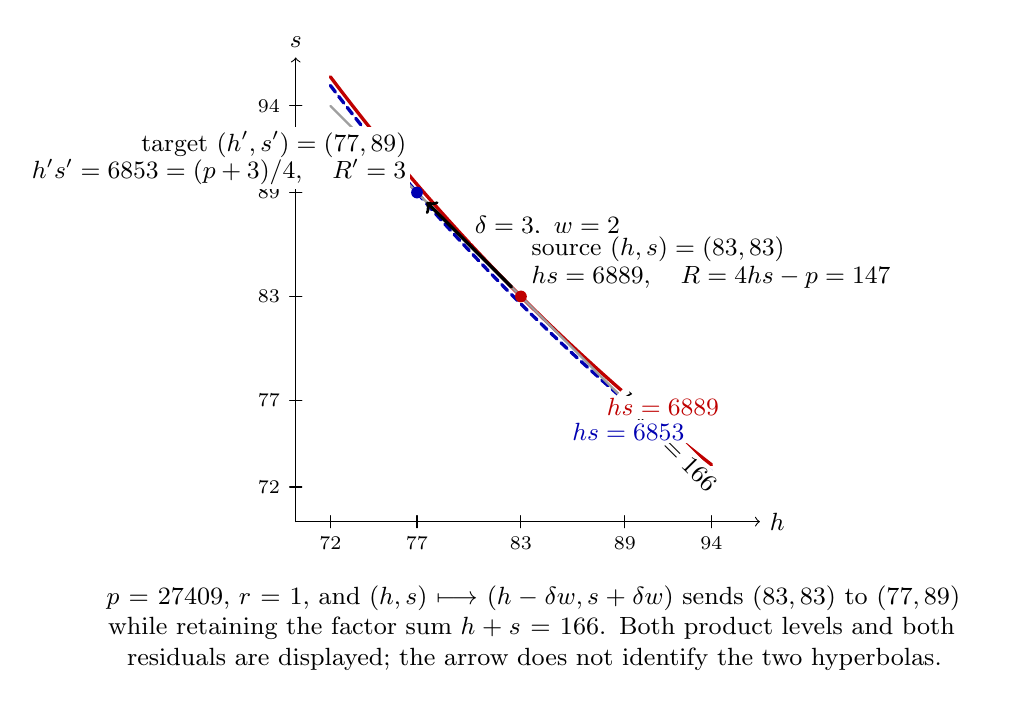
\begin{tikzpicture}[font=\small,line cap=round,line join=round]
  \begin{scope}[x=0.22cm,y=0.22cm,xshift=-15.4cm,yshift=-15.4cm]
    \draw[->] (70,70) -- (96.8,70) node[right] {$h$};
    \draw[->] (70,70) -- (70,96.8) node[above] {$s$};
    \foreach \x in {72,77,83,89,94}{
      \draw (\x,70.35) -- (\x,69.65)
        node[below] {\scriptsize $\x$};
      \draw (70.35,\x) -- (69.65,\x)
        node[left] {\scriptsize $\x$};
    }

    \draw[red!75!black,very thick]
      plot[domain=72:94,samples=100]
      (\x,{6889/\x});
    \draw[blue!70!black,very thick,densely dashed]
      plot[domain=72:94,samples=100]
      (\x,{6853/\x});
    \draw[gray!75,thick]
      plot[domain=72:94,samples=2]
      (\x,{166-\x});

    \fill[red!75!black] (83,83) circle[radius=0.34];
    \fill[blue!70!black] (77,89) circle[radius=0.34];
    \draw[->,black,very thick]
      (82.45,83.55) -- (77.55,88.45)
      node[midway,above right,fill=white,inner sep=1.5pt]
      {$\delta=3,\ w=2$};

    \node[above right,align=left,fill=white,inner sep=1.5pt]
      at (83.35,83.2)
      {$\text{source }(h,s)=(83,83)$\\[-1pt]
       $hs=6889,\quad R=4hs-p=147$};
    \node[above left,align=right,fill=white,inner sep=1.5pt]
      at (76.65,89.15)
      {$\text{target }(h',s')=(77,89)$\\[-1pt]
       $h's'=6853=(p+3)/4,\quad R'=3$};
    \node[rotate=-45,fill=white,inner sep=1pt]
      at (91.4,74.6) {$h+s=166$};
    \node[red!75!black,fill=white,inner sep=1pt]
      at (91.2,76.6) {$hs=6889$};
    \node[blue!70!black,fill=white,inner sep=1pt]
      at (89.2,75.2) {$hs=6853$};
  \end{scope}

  \node[align=center,text width=0.92\linewidth]
    at (3.0,-1.35)
    {$p=27409$, $r=1$, and
     $(h,s)\longmapsto(h-\delta w,s+\delta w)$ sends
     $(83,83)$ to $(77,89)$ while retaining the factor sum $h+s=166$.
     Both product levels and both residuals are displayed; the arrow does not
     identify the two hyperbolas.};
\end{tikzpicture}
\caption{The exact factor-sum arrow
$(h,s)\mapsto(h-\delta w,s+\delta w)$ on the first Pell-family example.
The source lies on $hs=6889$ and the target lies on $hs=6853$; their common
line is $h+s=166$.}
\label{fig:factor-sum-geometry}
\end{figure}


\subsection*{An exact mixed-channel arithmetic defect}
Write $R=KD$, where
$K=\prod\ell^{\lceil v_\ell(R)/2\rceil}$ and $D=R/K$.
The ideal $K\mathbb Z/R\mathbb Z$ has square zero. With
$\beta_\ell=v_\ell(u)-v_\ell(a)$ and $\eta=1$ for E, $0$ for M,
a trace has the unique coordinate
\[
 p^\eta u/a=-1+Kc\pmod R,\qquad c\in\mathbb Z/D.
\]
Its full gate is $c=0$, and its tail denominator is $D/\gcd(D,c)$.
For traces indexed by $j$, any integers $n_j$ with odd sum $N$, exact
channel exponent $\sum n_j\eta_j\in\{0,1\}$, and retained bounded vector
$\sum n_j\beta^{(j)}$ produce the original word
\[
 u_*=a^{1-N}\prod u_j^{n_j},\qquad c_*=\sum n_jc_j\pmod D.
\]
The proof is the finite identity
$\prod(1-Kc_j)^{n_j}=1-K\sum n_jc_j$, valid even for negative powers.
The exponent-box condition is indispensable: a unit residue alone is not a
new integer divisor.

At $(p,a,R)=(48049,12019,27)$, the proper trace words
\[
 (E,29189,c=1),\qquad(E,119,c=2),\qquad(M,707,c=1)
\]
have no individual fixed-word or fixed-ray divisor deletion. The signed
combination E$_1-$E$_2+$M is nevertheless an available M word
$173417$, with $c=0$, and gives
\[
 \frac4{48049}=\frac1{12019}+\frac1{22871324}+\frac1{330000532}.
\]
The full paper partitions every original box into finite cyclic coefficient
polynomials and proves a sharp saturation threshold, without replacing
bounded exponents by their generated subgroup.

\begin{figure}[htbp]
\centering
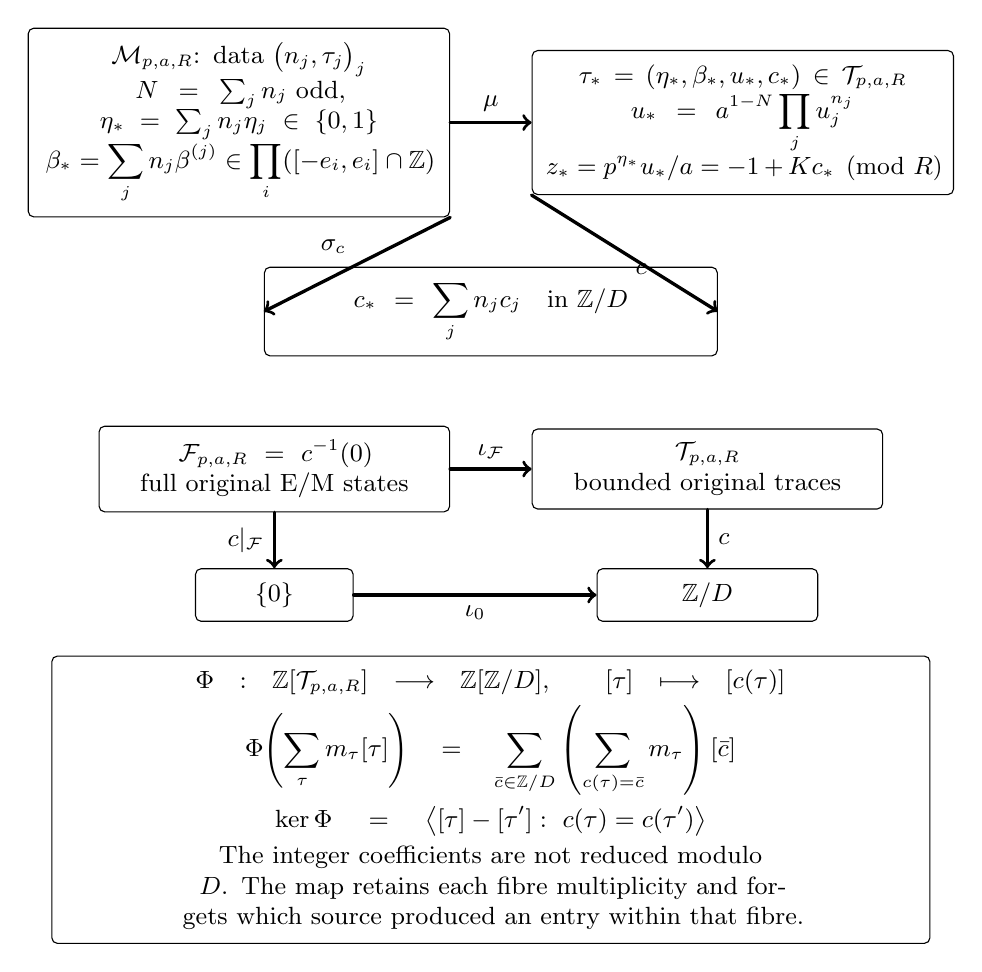
\begin{tikzpicture}[
  font=\small,
  box/.style={draw,rounded corners=2pt,align=center,inner sep=5pt},
  every path/.style={line cap=round,line join=round}
]
  \node[box,text width=5.0cm] (mix) at (-3.2,4.35)
    {$\mathcal M_{p,a,R}$: data $\bigl(n_j,\tau_j\bigr)_j$\\
     $N=\sum_j n_j$ odd,\quad
     $\eta_*=\sum_jn_j\eta_j\in\{0,1\}$\\
     $\displaystyle
       \beta_*=\sum_jn_j\beta^{(j)}
       \in\prod_i([-e_i,e_i]\cap\mathbb Z)$};
  \node[box,text width=5.0cm] (trace-star) at (3.2,4.35)
    {$\tau_*=(\eta_*,\beta_*,u_*,c_*)
       \in\mathcal T_{p,a,R}$\\
     $\displaystyle u_*=a^{1-N}\prod_j u_j^{n_j}$\\
     $z_*=p^{\eta_*}u_*/a=-1+Kc_*\pmod R$};
  \node[box,text width=5.4cm] (defect-sum) at (0,1.95)
    {$\displaystyle c_*=\sum_jn_jc_j\quad\hbox{in }\mathbb Z/D$};

  \draw[->,very thick] (mix) -- node[above]
    {$\mu$} (trace-star);
  \draw[->,very thick] (mix.south east) -- node[above left]
    {$\sigma_c$} (defect-sum.west);
  \draw[->,very thick] (trace-star.south west) -- node[below right]
    {$c$} (defect-sum.east);

  \node[box,text width=4.1cm] (full) at (-2.75,-0.05)
    {$\mathcal F_{p,a,R}=c^{-1}(0)$\\
     full original E/M states};
  \node[box,text width=4.1cm] (traces-fibre) at (2.75,-0.05)
    {$\mathcal T_{p,a,R}$\\bounded original traces};
  \node[box,text width=1.65cm] (zero) at (-2.75,-1.65)
    {$\{0\}$};
  \node[box,text width=2.45cm] (defect-fibre) at (2.75,-1.65)
    {$\mathbb Z/D$};
  \draw[->,very thick] (full) -- node[above]
    {$\iota_{\mathcal F}$} (traces-fibre);
  \draw[->,very thick] (full) -- node[left]
    {$c|_{\mathcal F}$} (zero);
  \draw[->,very thick] (traces-fibre) -- node[right]
    {$c$} (defect-fibre);
  \draw[->,very thick] (zero) -- node[below]
    {$\iota_0$} (defect-fibre);

  \node[box,text width=10.8cm] (module) at (0,-4.25)
    {$\displaystyle
      \Phi:\mathbb Z[\mathcal T_{p,a,R}]
      \longrightarrow\mathbb Z[\mathbb Z/D],\qquad
      [\tau]\longmapsto[c(\tau)]$\\[3pt]
     $\displaystyle
      \Phi\!\left(\sum_{\tau}m_\tau[\tau]\right)
      =\sum_{\bar c\in\mathbb Z/D}
       \left(\sum_{c(\tau)=\bar c}m_\tau\right)[\bar c]$\\[3pt]
     $\displaystyle
      \ker\Phi=
      \left\langle[\tau]-[\tau']:\ c(\tau)=c(\tau')\right\rangle$\\[2pt]
     The integer coefficients are not reduced modulo $D$.
     The map retains each fibre multiplicity and forgets which source produced
     an entry within that fibre.};
\end{tikzpicture}
\caption{Typed maps for the defect equation
$p^\eta u/a=-1+Kc\pmod R$.  In the upper triangle,
$\sigma_c((n_j,\tau_j)_j)=\sum_jn_jc_j$, and the triangle commutes by the
mixed integer-exponent law.  The middle square identifies the
full states as the zero fibre.  The lower map states the exact kernel and the
information lost when original trace words are replaced by their defect-bin
coefficient vector.}
\label{fig:defect-map}
\end{figure}


\subsection*{The distinct fixed-tail-sum fibre}
The factor-sum arrow above retains $h+s$.  Fixing instead the numerical tail
sum $Y+Z=N$ gives a different exact problem.  Put
\[
 \mathcal D=N(N-p),\qquad \rho=4A-p,\qquad \Delta=Z-Y.
\]
The ordered positive integer triples with $p/4<A<p/2$ and
\[
 \frac4p=\frac1A+\frac1Y+\frac1Z,\qquad Y+Z=N
\]
are in bijection with
\[
 \rho\mid N,\quad 0<\rho<p,\quad \rho\equiv-p\pmod4,\quad
 \Delta^2=\mathcal D-\frac{Np^2}{\rho},\quad
 |\Delta|<N,\quad \Delta\equiv N\pmod2.
\]
The inverse is
\[
 (A,Y,Z)=\left(\frac{p+\rho}{4},\frac{N-\Delta}{2},
                    \frac{N+\Delta}{2}\right).
\]
Indeed the reciprocal identity gives
$YZ=Np(p+\rho)/(4\rho)$, hence
$\rho\Delta^2=N((N-p)\rho-p^2)$.  Since $p$ is prime and $0<\rho<p$,
this forces $\rho\mid N$.  The displayed inverse proves sufficiency.

Writing $\rho=\delta v^2$ and $X=v\Delta$ gives the exact lattice equation
\[
 X^2-\mathcal Dv^2=-\frac{Np^2}{\delta},\qquad
 \delta v^2\mid N,\qquad X\equiv Nv\pmod{2v}.
\]
The divisibility and congruence gates are essential.  Equivalently, if
$B=\rho Y-pA$, $C=\rho Z-pA$, $w=B-C$, then
\[
 (2\mathcal D\rho-p^2N)^2-\mathcal D(2w)^2=p^4N^2,
\]
but integer tails additionally require $\rho\mid w$.

\begin{theorem}[Prime-square fixed-sum divisor obstruction]
Let $p,q$ be odd primes with $p\equiv1\pmod4$ and
$2q^2<p<4q^2$, and set $R=4q^2-p$.  Choose $u=q$ or $q^3$ and
an E/M channel.  If its prime-square source is a proper trace, then no
positive integral target with the same numerical tail sum $N$ has residual
$S=4A-p$ satisfying $S\mid R$ and $0<S<R$.
\end{theorem}
\begin{proof}
Put $G_E(u)=4u+1$ and $G_M(u)=p+4u$.  In the four cases define
\[
\begin{array}{c|c|c}
(E,q)&H=p+q&N=qH^2/R\\
(E,q^3)&H=pq+1&N=qH^2/R\\
(M,q),(M,q^3)&H=q+1&N=pqH^2/R.
\end{array}
\]
The identities
\[
H=qG_E(q)-R,\quad H=G_E(q^3)-qR,\quad
G_M(q)=4qH-R,\quad G_M(q^3)=qR+pH
\]
show that properness is $R\mid H^2$ and $R\nmid H$.
Let
\[
g=(R,H),\quad \eta=R/g,\quad F=H/g,\quad k_0=g/\eta.
\]
Then
\[
R=k_0\eta^2,\quad H=k_0\eta F,\quad
(\eta,F)=1,\quad\eta\ge3,
\]
with $(pq,k_0F)=1$, and
\[
N=qk_0F^2\quad(E),\qquad N=pqk_0F^2\quad(M),\qquad
(R,N)=k_0.
\]

Suppose a target exists.  The exact inequalities are
\[
A=\frac{p+S}{4}<\frac{p+R}{4}=q^2<\frac p2.
\]
Moreover $S\equiv3\pmod4$.  From $SYZ=NpA$ and
$(S,pA)=1$ one gets $S\mid N$, hence $S\mid k_0$.
Factoring
\[
(SY-pA)(SZ-pA)=(pA)^2
\]
with the $p$-valuation pair retained shows, up to the E tail orientation,
that every target is exactly one of
\[
\begin{array}{c|c|c}
E&S\kappa=pr+s&N=hS\kappa^2\\
M&S\lambda=r+s&N=phS\lambda^2,
\end{array}
\qquad A=hrs,\quad(r,s)=1.
\]
Thus the parity of $v_p(N)$ forces the target into the source channel.
Writing $\theta=\kappa$ in E and $\theta=\lambda$ in M gives
\[
q\frac{k_0}{S}F^2=h\theta^2.
\]
Since $q\nmid(k_0/S)F$ and $h\mid A<q^2$, one has
$h=qh_0$.  Hence
\[
A=q(q-j),\quad0<j<q,\quad R-S=4qj,\qquad
\frac{k_0}{S}F^2=h_0\theta^2.
\]

For $(E,q)$, the gate $S\kappa=pr+s>p$ contradicts
\[
S\kappa\le F\sqrt{Sk_0}\le Fk_0
=\frac{p+q}{\eta}<p.
\]
For either M orientation, $q=k_0\eta F-1$; here $k_0,\eta$ are odd and
$F$ is even.  Moreover
\[
k_0\eta(\eta-4jF)=S-4j.
\]
Here $S-4j$ is nonzero, while
$0<S<k_0\eta$ and
$0<4j<(k_0\eta^2)/q<k_0\eta$ because
$q\ge2\eta-1>\eta$.  This is impossible for a nonzero multiple of
$k_0\eta$.

It remains to treat $(E,q^3)$.  Write
$F=nw$, $\kappa=mw$, $(m,n)=1$.  There is a positive $\tau$ such that
\[
k_0/S=\tau m^2,\qquad h_0=\tau n^2.
\]
With $\Gamma=\tau m\eta n$,
\[
pq+1=k_0\eta F=\Gamma S\kappa=\Gamma(pr+s),
\]
so $\Gamma s\equiv1\pmod p$.  Also
\[
0<\tau ns=\frac{q-j}{nr}<q.
\]
Finally $R=S\tau(m\eta)^2<2q^2$, and $S\ge3$, so
$m\eta<q$.  Therefore
$0<\Gamma s<q^2<p$, forcing $\Gamma s=1$, contrary to
$\Gamma s\ge\eta\ge3$.
\end{proof}

The divisor condition is essential to the theorem: it leaves open residuals
$S<R$ with $S\nmid R$, and changing $N$ is outside this fibre.

For the proper trace
\[
 (p,a,R,u,h,r,s)=(67369,16849,27,1421,29,7,83),\qquad
 N=586110300,
\]
one has
\[
 (B,C,w)=(13459046189,95731349,13363314840),\qquad
 w\equiv18\pmod{27}.
\]
The only residual candidates are $3,15,75,87,435,2175$.  The first has
negative discriminant; the other discriminants are respectively $2$ modulo
$3$, $5$ modulo $7$, $2$ modulo $3$, $3$ modulo $7$, and $2$ modulo $3$.
Thus none is a square.  The complete first-half certificate treats all 69
proper trace tags at this prime: their 51 distinct sums yield 507 eligible
residuals, 478 nonnegative discriminants, and no integral target.  This is a
fixed-sum obstruction, not an ES counterexample and not an obstruction to the
different factor-sum arrow.

\subsection*{A precise limitation on descent}
The source-changing rules above do not apply to every trace. A separate,
exhaustive standard-library certificate proves that $67369$ is the least
prime $1\bmod24$ for which the first trace shell is earlier than every full
shell. Its first trace has $a=16849$, $R=27$; its first full gate has $a=16850$,
$R=31$. All 817 primes in the stated class through that bound and all their
shells through first full occupancy are replayed by two implementations.
Hence a universal repair from \emph{every} trace cannot require $a'\le a$.
This is an obstruction to a proposed termination invariant, not an ES
counterexample. Universal occupancy of the full original source is still
unproved.

\begin{thebibliography}{9}
\bibitem{ET} C. Elsholtz and T. Tao (2013), Counting the number of solutions to
the Erd\H{o}s--Straus equation on unit fractions, \emph{J. Aust. Math. Soc.}
94, 50--105. \href{https://arxiv.org/abs/1107.1010}{arXiv:1107.1010v6},
\S2, Propositions 2.2 and 2.6, equations (2.13)--(2.22).
\bibitem{Yam} K. Yamamoto (1965), On the Diophantine equation
$4/n=1/x+1/y+1/z$, \emph{Mem. Fac. Sci. Kyushu Univ. A} 19, 37--47.
Lemma 2, equation (4), p.~38. doi:10.2206/kyushumfs.19.37.
\bibitem{Work} The Clankers (2026), \emph{Bounded additive gate defects and a
Pell return for Erd\H{o}s--Straus trace sources}, accompanying complete proof,
standard-library verifier, separate checker and JSON certificates.
Based on Erd\H{o}s--Straus Foundation revision
\texttt{20709bee872ad10e4cc7d7b976d975e24532a803}.
No historical-priority determination, independent human review or Lean build
is claimed.
\end{thebibliography}
\end{document}
